\newcommand{\bmath}[1]{\mbox{$\mathbf{#1}$}}
\newcommand{\q}{\bmath{q}}
\newcommand{\y}{\bmath{y}}
\newcommand{\x}{\bmath{x}}
\newcommand{\de}{\bmath{d}}
\newcommand{\ere}{\bmath{r}}
\newcommand{\omegav}{\bmath{\omega}}
\newcommand{\f}{\bmath{f}}
\newcommand{\n}{\bmath{n}}
\newcommand{\Pe}{\bmath{P}}
\newcommand{\F}{\bmath{F}}
\newcommand{\G}{\bmath{G}}
\newcommand{\I}{\bmath{I}}
\newcommand{\J}{\bmath{J}}
\newcommand{\K}{\bmath{K}}
\newcommand{\Ese}{\bmath{S}}
\newcommand{\R}{\bmath{R}}
\newcommand{\Ha}{\bmath{H}}
\newcommand{\h}{\bmath{h}}
\newcommand{\m}{\bmath{m}}
\newcommand{\z}{\bmath{z}}
\newcommand{\uve}{\bmath{v}}
\newcommand{\V}{\bmath{V}}
\newcommand{\undist}{\bmath{uds}}
\newcommand{\dist}{\bmath{ds}}
\newcommand{\amin}{\bmath{a}}

\documentclass[a4paper,12pt]{article}

\usepackage{times,epsfig}


\setlength{\oddsidemargin}{-7mm}
\setlength{\evensidemargin}{-7mm}
\setlength{\topmargin}{-14mm}
\setlength{\parindent}{0mm}
\setlength{\parskip}{1mm}
\setlength{\textwidth}{173mm}
\setlength{\textheight}{244mm}
\setlength{\unitlength}{1mm}

%\input newcom.tex
%\input symbols.tex


\newcommand{\coursetitle}{SLAM Summer School 2006}
\newcommand{\tutorialtitle}{Practical 2: SLAM using Monocular Vision}
\newcommand{\docauthor}{Javier Civera, University of Zaragoza\\
                        Andrew J. Davison, Imperial College London\\
                        J.M.M Montiel, University of Zaragoza.}
\newcommand{\docemails}{josemari@unizar.es, jcivera@unizar.es, ajd@doc.ic.ac.uk}


\begin{document}


\bibliographystyle{plain}


\begin{center}

\hrule
\vspace{2mm}
{\LARGE\bf \coursetitle}

\vspace{2mm}
{\Large\bf \tutorialtitle}

\vspace{2mm}
{\large \docauthor}
\\
{\large \texttt{\docemails}}


\end{center}


\hrule

%\hrule
\vspace{5mm}



%\vspace{10mm}
%\hrule
%\vspace{2mm}

\setcounter{page}{1}
\setcounter{section}{0}



\section{Objectives}
\begin{enumerate}
\item Understanding the characteristics of efficient (potentially
real-time) SLAM using a monocular
camera as the only sensor.
\begin{enumerate}
\item Map management.
\item Feature initialization.
\item Near and far features.
\end{enumerate}
\item Understanding the inverse depth parametrization of map
features in monocular SLAM.
\item Understanding the performance
limits of a constant velocity motion model for a camera when no odometry is available.
\end{enumerate}


\section{Exercise 1. Feature selection and matching.}
One of the characteristics of vision-based SLAM is that there is too
much information in an image sequence for
current computers to process in real-time. We therefore use heuristics to select which features to
include in the map. The desirable properties of map
features are:
\begin{enumerate}
\item Saliency: features have to be identified by distinct texture patches.
\item A minimum number (e.g. 14) should  be visible in the image at all times --- when this is not the case, 
new map features are initialized.
\item The features should be spread over the whole image.
\end{enumerate}

The goal of this exercise is to manually initialize features
in order to meet the above criteria, and to understand better how an
automatic initialization algorithm should work. Run
\texttt{mono\_slam.m}. With the user interface, you can add
features and perform step by step EKF SLAM:
\begin{enumerate}
\item In the first image add about ten salient features spread over the image.
You can watch the movie \texttt{juslibol\_SLAM.mpg} (using for
instance \texttt{mpeg\_play} on a Unix workstation) as an example of how
to select suitable features (but you
can of course select other ones). This movie shows the results of
applying automatic feature selection.
\item As the camera moves, some features will leave the field of view, and you will
have to add new ones in order to maintain around 14 visible map features.
\end{enumerate}


\section{Exercise 2. Near features and far features.}
A camera is a bearing-only sensor. This means that the depth of a
feature cannot be estimated from a single image measurement. The
depth of the feature can be estimated only if the feature is
observed from different points of view --- and only if the camera
translates enough to produce significant parallax. In particular, it
may take a very long time to obtain accurate estimates of the depths
of distant features, since they display very little or no parallax
when the camera moves small distances.

The goal of this exercise is to observe the different
evolution of depth estimates in the cases of near and distant features
and the influence that this has on the
camera location estimate.

\begin{enumerate}
\item Open the video \texttt{parallax.mpg}.
      Observe the different motions \emph{in the image} of features at
different depths.
      Open the video \texttt{noparallax.mpg} (taken from a camera
which does not significantly translate) and observe that the
image  motion of features at different depths.
\item Now look at the video we are using for this practical (\texttt{juslibol.mpg}).
Distinguish which parts of the scene in this video contain
\emph{low parallax motion}.
\item Run \texttt{mono\_slam.m}.
\begin{itemize}
\item  Observe what happens to the features in the 3D map
(initialization value and covariance and value and covariance
after several frames). Red dots display the estimated values and red
lines bound $95\%$ probability regions denoting uncertainty.
\item The code singles out features \#5 and \#15 and displays their depth
estimates and $95\%$ probability regions: [lower limit,
estimation, upper limit]. When clicking, make sure that feature \#5
corresponds to a near one (for example, on the car) and feature \#15
corresponds to a far one (for example, the tree appearing on the
left).
\item   Notice the difference between the evolution of the estimates
of these near and
distant features.
\item Observe the evolution of the camera location uncertainty
(use the axes limit controls in the user interface).
\item Observe what happens to features and camera location uncertainties
in the low parallax motion part of the image sequence discussed above in 2. Notice
the difference between this part of the 3D map (constructed with
low parallax information) and the high parallax parts.
\end{itemize}
\end{enumerate}




\section{Exercise 3. Inverse depth parameterization.}

Initializing a feature in monocular SLAM is a challenging issue,
because the depth uncertainty is not well modelled by a Gaussian.
This problem is overcome using inverse depth instead of the
classical $XYZ$ representation.
\begin{figure}
\centering
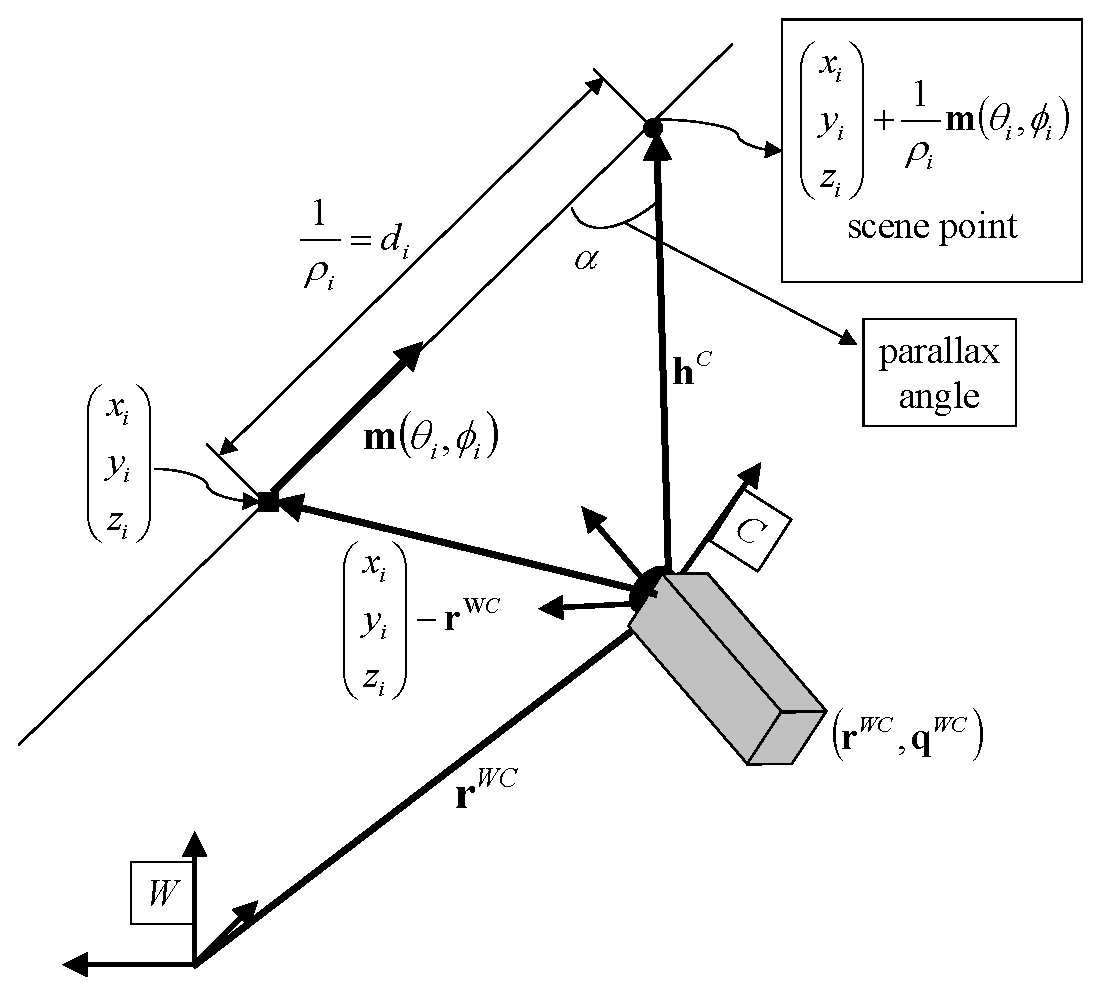
\includegraphics[width=0.5\columnwidth]{FeatureObservationAndParameterization.eps}
\caption{Feature parameterization and measurement equation.}
\label{fig_feat_par}
\end{figure}

The Matlab code of this practical uses the inverse depth
parametrization of feature positions. The total state
vector:
\begin{equation}
\x=\left(\x_v^\top, \y_1^\top, \y_2^\top, \ldots
\y_n^\top\right)^\top.
\end{equation}
is composed of:
\begin{enumerate}
\item 13 components that correspond to the location, orientation, and
velocity and angular velocity of
the camera:
\begin{equation}
\x_v=\left(\begin{array}{c}\ere^{WC}\\\q^{WC}\\\uve^{W}\\\omegav^{W}\end{array}\right).
\end{equation}

\item The rest of the components are features. Each feature is represented by 6 parameters;
 the position of the camera the first time the feature was
 seen $x_i,  y_i,  z_i$, a semi-infinite ray parametrized with azimuth-elevation angles ($\theta,\phi$), 
 and the inverse depth $\rho$ of the feature along the ray:
\begin{equation}
\y_i=\left(\begin{array}{cccccc}x_i & y_i & z_i & \theta_i &
\phi_i & \rho_i\end{array}\right)^\top
~.
\end{equation}
So the transformation from the inverse depth parametrization to a
standard 
Euclidean system is:
\begin{equation}
\left(\begin{array}{c}x\\y\\z\end{array}\right)=\left(\begin{array}{c}x_i\\y_i\\z_i\end{array}\right)+
                    \frac{1}{\rho_i}\m\left(\theta_i,
                    \phi_i\right).
\end{equation}
where:
\begin{equation}
\m=\left(\begin{array}{ccc}\cos\phi_i \sin\theta_i&
                     -\sin\phi_i&
                     \cos\phi_i \cos\theta_i\end{array}\right)^\top
                     \label{eq-m}
~.
\end{equation}

\end{enumerate}
The goal of this exercise is to understand the inverse depth
parametrization.
\begin{enumerate}
\item The code stores partial information about features \#5 and
\#15 in the file \texttt{history.mat}:

\begin{itemize}
\item \texttt{feature5History} is a 6 row matrix, each column containing the feature \#5
location coded in inverse depth at step $k$.
\item \texttt{rhoHistory\_5} is a row vector containing the inverse depth estimation
history for feature 5.
\item \texttt{rhoHistory\_15} is a row vector containing the inverse depth estimation
history for feature 15.
\item \texttt{rhoStdHistory\_5} is a row vector containing the inverse depth
standard deviation history for feature 5.
\item \texttt{rhoStdHistory\_15} is a row vector containing the inverse depth standard deviation
history for feature 15.
\end{itemize}

\item Compute the $XYZ$ Euclidean location for feature \#5 after
processing all the images.

\item Do a graph with the value of the inverse depth and the
  $95\%$ acceptance region history for both features \#5 and \#15.
  Use the matlab functions \texttt{open}, \texttt{figure}, \texttt{hold}, and \texttt{plot}.
  Comment on the difference between the two graphs.

\item After processing the whole sequence, what are the estimates and the
uncertainty regions \emph{expressed in depth} for both features?

Think about a feature at infinity ---  what inverse depth would it have?

In the graphs, are there regions where infinity is included within the
uncertainty bounds as a possible depth for each feature? The inverse
depth parametrization is particularly valuable in being able to
represent the possibility of features at infinity.


\end{enumerate}

\section{Exercise 4. Constant velocity motion model (optional)}
Monocular SLAM uses a camera as the unique sensor, without any
odometry input. A constant velocity model is instead used to model
approximately smooth motion of the camera. This model requires
parameters to be set defining the camera frame rate, and the maximum
expected angular and linear accelerations. These parameters together
determine how much uncertainty is added to the camera position and
orientation estimates during each motion prediction, and therefore
also determines the size of the uncertainty-guided search regions used
for feature matching. High expected accelerations or a low frame rate
will lead to large search regions.


The goal of this exercise is to analyse the effect of changing the linear
acceleration, the angular acceleration and frame rate parameters.

\begin{enumerate}
\item The initial linear and angular acceleration tunings are $6\frac{m}{s^2}$ and $6\frac{\mbox{rad}}{s^2}$.
\item Increase the angular acceleration only (for instance, double
the value) and analyse the effect on the search regions. Find this
parameter in the file \texttt{mono\_slam.m} (its name is
\texttt{sigma\_alphaNoise}).

\item Increase the linear acceleration only (for instance, double
the value), analyse the effect and compare what happens now. The name of this parameter is \texttt{sigma\_aNoise}.

\item Reduce the frame rate of processing to see what happens when only:
\begin{enumerate}
\item 1 out of 2 images
\item 1 out of 4 images
\end{enumerate}
are processed.

Clue: find the variable step and the code associated with this
variable. You will also have to modify the variable
\texttt{deltat} which sets the time between frames.

Does the processing time has increase or decrease as the result of
processing less images? Can you explain this?


\end{enumerate}

\nocite{Hartley2004,Davison2003,Montiel2006RSS,Bar-Shalom-88}
\bibliographystyle{ieee}
\bibliography{IEEEabrv,practical}
\end{document}
